
%(BEGIN_QUESTION)
% Copyright 2010, Tony R. Kuphaldt, released under the Creative Commons Attribution License (v 1.0)
% This means you may do almost anything with this work of mine, so long as you give me proper credit

Sketch the necessary connecting tubes and wires to calibrate a DP transmitter to a low pressure range (somewhere in the range of a few inches of water), using a hand (bicycle-style) air pump as the pressure source and a U-tube manometer as a pressure standard.  As pressure increases, the transmitter's output signal should increase as well:

$$\includegraphics[width=15.5cm]{i00022x01.eps}$$

\vfil 

\underbar{file i00022}
\eject
%(END_QUESTION)





%(BEGIN_ANSWER)

This is a graded question -- no answers or hints given!

%(END_ANSWER)





%(BEGIN_NOTES)

This is just one solution -- others are possible:

$$\includegraphics[width=15.5cm]{i00022x02.eps}$$

The purpose of the air tank is to add volume to the system, so that each stroke of the hand pump adds less pressure to the system.  If you have ever tried to pump up an automobile tire using a bicycle pump, you understand this principle well: it takes {\it lots} of pump strokes to inflate a car tire, but relatively few to inflate a bicycle tire, due to the vast difference in volumes between the two types of tires.  We're intentionally adding volume to this system in order to exploit the principle and thereby make each pump stroke less influential.  

If not for the air tank, just one stroke of the hand pump would likely generate enough pressure to completely blow all the water out of the manometer!

\vfil \eject

A very common mistake made by students is to connect the manometer in ``series'' between the air pump and the tank, like this:

$$\includegraphics[width=15.5cm]{i00022x03.eps}$$

If one were to connect a manometer in this manner, it would register the {\it difference} in air pressure between the air pump and the tank rather than register the (gauge) air pressure in the tank as it should.  What we want is a system where the air pump's output gets sent to the tank with nothing in between to interfere with the air reaching its destination, and the manometer senses the pressure difference between the tank and the ambient atmospheric pressure.  Connected improperly, we would never expect the manometer's reading to agree with the pressure transmitter's reading except by chance.

This mistake would be analogous to connecting a voltmeter (an electrical ``pressure'' sensing device) in series between a voltage source (air pump) and a capacitor (tank) like this.  As with the improperly plumbed manometer, we would have no reason to expect these two voltmeters to agree:

$$\includegraphics[width=15.5cm]{i00022x04.eps}$$


%INDEX% Calibration, generating low air pressures using a bicycle (hand) pump

%(END_NOTES)


